\documentclass{report}
\usepackage{graphicx, color}
\usepackage[a4paper,margin=2cm]{geometry}
\usepackage{lipsum}

\newcommand{\red}[1]{{\color{red}{#1}}}

\usepackage{amsmath,cite,url}
\usepackage{graphicx}
\usepackage{color,soul}

% packages
\usepackage{amssymb}
\usepackage{bbm}
\usepackage[colorinlistoftodos,prependcaption,textsize=tiny]{todonotes}
\usepackage{subcaption}
\usepackage{booktabs}
% TODO [JAB]: If you don't like Times Math, take this out. It does look a little funny for equations (although it matches Microsoft Word better), but it also makes in-text math look *much* more consistent.
% \usepackage{newtxmath}

% custom commands
\DeclareRobustCommand{\diffword}[1]{{\sethlcolor{orange}\hl{#1}}}
% \DeclareRobustCommand{\diffword}[1]{#1}}
\newcommand{\beginsupplement}{%
    \setcounter{table}{0}
    \renewcommand{\thetable}{S\arabic{table}}%
    \setcounter{figure}{0}
    \renewcommand{\thefigure}{S\arabic{figure}}%
}

\newcommand{\ra}[1]{\renewcommand{\arraystretch}{#1}}



\begin{document}

\begin{titlepage}

\newcommand{\HRule}{\rule{\linewidth}{0.5mm}} % Defines a new command for the horizontal lines, change thickness here
\center % Center everything on the page
 
%----------------------------------------------------------------------------------------
%	HEADING SECTIONS
%----------------------------------------------------------------------------------------


\includegraphics[width=\linewidth]{images/uva.jpeg}\\[2.5cm]
\textsc{\Large MSc Artificial Intelligence}\\[0.2cm]
% \textsc{\normalsize Track: \red{track}}\\[1.0cm] % track
\textsc{\Large Master Thesis}\\[0.5cm] 

%----------------------------------------------------------------------------------------
%	TITLE SECTION
%----------------------------------------------------------------------------------------

\HRule \\[0.4cm]
{ \huge \bfseries Contrastive Learning of Musical Representations}\\[0.4cm] % Title of your document
\HRule \\[0.5cm]
 
%----------------------------------------------------------------------------------------
%	AUTHOR SECTION
%----------------------------------------------------------------------------------------

by\\[0.2cm]
\textsc{\Large J. Spijkervet}\\[0.2cm] %you name
10879609\\[1cm]


%----------------------------------------------------------------------------------------
%	DATE SECTION
%----------------------------------------------------------------------------------------

{\Large \today}\\[1cm] % Date, change the \today to a set date if you want to be precise

Number of Credits\\ %
48\\[1cm]%

%----------------------------------------------------------------------------------------
%	COMMITTEE SECTION
%----------------------------------------------------------------------------------------
\begin{minipage}[t]{0.4\textwidth}
\begin{flushleft} \large
\emph{Supervisor:} \\
dr. J.A. \textsc{Burgoyne}% Supervisor's Name
\end{flushleft}
\end{minipage}
~
\begin{minipage}[t]{0.4\textwidth}
\begin{flushright} \large
\emph{Assessor:} \\
\red{Dr A  \textsc{Person}}\\
\end{flushright}
\end{minipage}\\[2cm]

%----------------------------------------------------------------------------------------
%	LOGO SECTION
%----------------------------------------------------------------------------------------

% \framebox{\rule{0pt}{2.5cm}\rule{2.5cm}{0pt}}\\[0.5cm]
%\includegraphics[width=2.5cm]{figure}\\ % Include a department/university logo - this will require the graphicx package
\textsc{Faculteit der Natuurkunde, Wiskunde en Informatica}\\[1.0cm]
\textsc{\large University of Amsterdam}\\[1.0cm] % 
 
%----------------------------------------------------------------------------------------

\vfill % Fill the rest of the page with whitespace

\end{titlepage}


\begin{abstract}
    Learning and designing mid-level representations lie at the heart of many successful machine learning tasks. Supervised approaches have seen widespread adoption within music information retrieval for learning such representations, but unsupervised representation learning remains challenging. We propose a self-supervised contrastive learning framework that learns useful, compact and robust representations from high-dimensional, raw audio data. Using techniques from contrastive predictive coding, we formulate the learning objective on correlated, augmented training examples directly in the latent space. Furthermore, we show that the autoregression inherent to contrastive predictive coding is not essential for learning effective representations; learning mostly depends on the composition of data augmentations. Our framework requires no manual labeling, no fine-tuning and no pre-processing of the input data. Moreover, we show that the learned representations are transferable across different corpora (the McGill Billboard, GTZAN and Free Music Archive datasets), indicating that they capture and generalise important musical knowledge. We evaluate the representations using a music classification task on the MagnaTagATune dataset. State-of-the-art, supervised end-to-end models achieve an ROC-AUC score of 89\% with 2.5 million parameters. Using our mid-level representations and basic logistic regression, we achieve a score of 87\% with 100 times fewer parameters.
\end{abstract}

\renewcommand{\abstractname}{Acknowledgements}
\begin{abstract}

\end{abstract}

\tableofcontents

\chapter{Introduction}
The field of music information retrieval has seen many successes since the emergence of deep learning. Supervised, end-to-end learning methods have been widely used in tasks like chord recognition \cite{korzeniowski_fully_2016, chen_harmony_2019}, key detection \cite{korzeniowski_end--end_2017}, beat tracking \cite{bock_joint_2016}, music audio tagging \cite{pons_end--end_2017} and music recommendation \cite{van_den_oord_deep_2013}. These methods use labeled corpora, which are hard\cite{doi:10.1080/09298215.2019.1613436}, expensive and time-consuming to create, while raw unlabeled musical data is available in vast amounts. Despite the importance of unsupervised learning in MIR for raw, high-dimensional signals of audio, it has yet to see breakthroughs similar to supervised learning. It has enjoyed successes with methods like PCA, PMSC's and spherical $k$-means that rely on a transformation pipeline\cite{hamel2011temporal, dieleman_feature_learning}, but learning effective representations of raw audio remains elusive. 

\begin{figure}[t]
    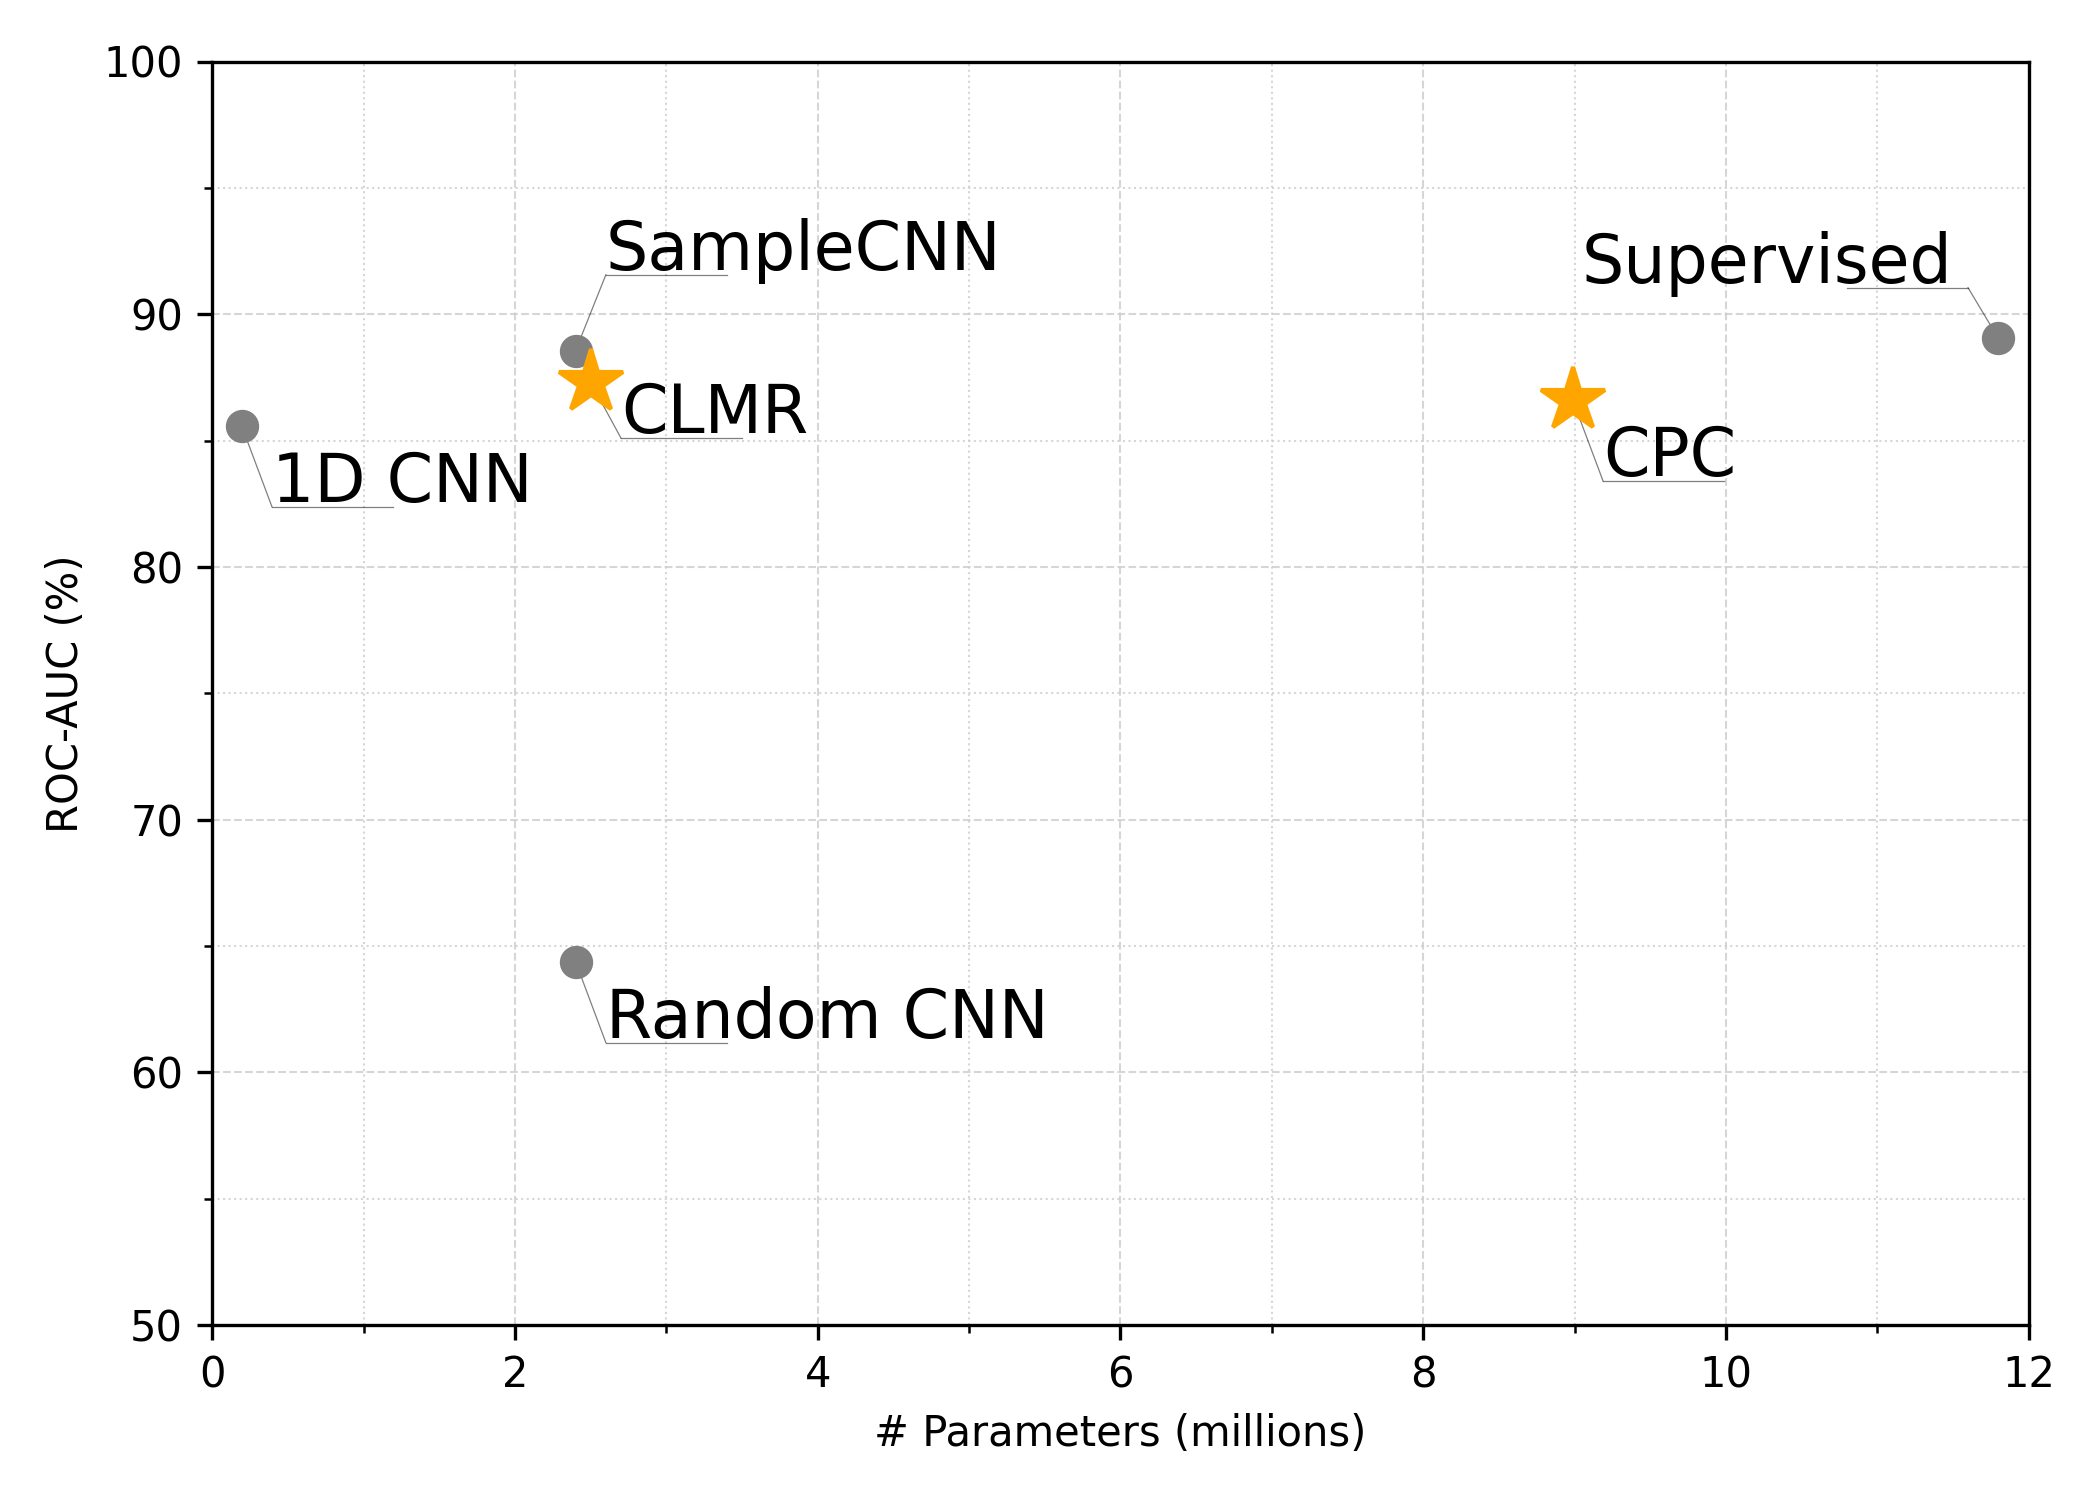
\includegraphics[width=\columnwidth]{figs/performance.png}
    \caption{Performance and model complexity comparison of supervised models (grey) and self-supervised models (ours) in music classification of raw audio waveforms on the MagnaTagATune dataset to evaluate musical representations. Supervised models were trained end-to-end, while CLMR and CPC are pre-trained without ground truth: their scores are obtained by training a linear, logistic regression classifier on their learned representations but nonetheless perform practically identically to the supervised models.}
    \label{fig:example}
\end{figure}

Self-supervised representation learning, a form of unsupervised learning, is a relatively new, upcoming learning paradigm\cite{dosovitskiy2015discriminative, oord_representation_2019, hjelm_learning_2019,chen_simple_2020}.
The general goal of representation learning is to train a function $g$ that maps input data $x \in \mathbb{R}^d$ to some representation of lower dimensionality, while preserving as much useful information as possible. In the absence of ground truth, there can be no ordinary loss function for training $g$; self-supervised learning trains by way of a proxy loss function instead, obtained by withholding or augmenting parts of the input data. One way to preserve the amount of useful information during self-supervised learning is to define the proxy loss function with respect to a relatively simple `pretext' task, with the idea that a representation that is good for the pretext task will also be useful for other tasks. Many approaches simply rely on heuristics to design pretext tasks\cite{doersch_unsupervised_2015,zhang2016colorful}, e.g., by defining pitch transformation as a pretext\cite{spice}. Alternatively, \emph{contrastive representation learning} formulates the proxy loss directly on the learned representations and relies on comparing and contrasting multiple, slightly differing versions of any one example. The rationale behind this contrastive strategy is \emph{predictive coding}, a theory that the human brain encodes causal structures and predicts future events at different levels of abstraction\cite{friston_predictive_2009}.


% may want to zoom out a bit, from 50 - 100 y-axis
% put in parenthesis [ours]
% square brackets citation
% add random baseline at 60% ROC
% add a labeled bracket that indicates the penalty / cost -> self-supervision penalty
% make the point of self-supervised learning this way

In this paper we introduce two models for self-supervised, contrastive representation learning of raw audio waveforms of music. %To demonstrate their effectiveness,
The models are evaluated on a music tagging task, enabling us to evaluate their versatility: music tags describe many characteristics of music, e.g., genre, instrumentation and dynamics. Our key contributions are summarized as follows.
\begin{itemize}
    \item The models achieve strong performance on the music classification task, despite unsupervised contrastive training (see Figure~\ref{fig:example}).
    \item The models learn useful, compact representations from raw signals of musical audio.
    \item The learned representations are transferable across different musical corpora.
    \item The proposed models can learn from \emph{any} dataset of raw audio, requiring neither transformations nor fine-tuning on the input data; nor do the models require manually annotated labels for pre-training.
\end{itemize}



\chapter{Background}
The performance of machine learning models is heavily dependent on the choice of features and representations. These features are often engineered using human intuition and domain knowledge of the composition of the input data (i.e., feature engineering). While feature engineering can greatly help to improve model performance, it is time-consuming and highlights the inability of traditional learning algorithms to identify and disentangle explanatory factors hidden in high-dimensional signals. 

\section{Representation Learning}

The goal of representation learning is to identify features that make  prediction tasks easier and more robust to the complex variations of natural data\cite{bengio2013representation}. Supervised techniques for representation learning have now been successfully applied to a variety of tasks \cite{korzeniowski_fully_2016, chen_harmony_2019, korzeniowski_end--end_2017, bock_joint_2016, pons_end--end_2017, van_den_oord_deep_2013}. 
% In the unsupervised domain, generative modeling and likelihood-based models use reconstruction of the observations as the objective for learning useful representations of the data. 
In unsupervised representation learning, generative modeling and likelihood-based models typically find useful representations of the data by attempting to reconstruct the observations on the basis of their learned representations\cite{goodfellow2014generative, unsupervised_gan}.
In contrast to these unsupervised approaches, \emph{self-supervised} contrastive representation learning aims to identify the explanatory factors of the data using an objective that is formulated with respect to the learned representations directly.

Work on self-supervised learning in audio is still very limited. Contrastive predictive coding (CPC) as formulated by \cite{oord_representation_2019} is a universal approach to contrastive learning, and has been successful for speaker and phoneme classification, among other tasks. Recent advances have also been made in self-supervised pitch estimation\cite{spice}, closely matching supervised, state-of-the-art baselines despite being trained without ground truth labels. That work, however, relies on pre-processing with a CQT transform: to the best of our knowledge, we propose the first self-supervised learning framework for raw waveforms of musical audio. 

\subsection{Invariance and Levels of Abstraction}
Ideal feature representations should be invariant to local translations and noisy variations of the input signal while remaing sensitive to higher-level semantic information. Put differently, the main challenge is to learn representations that effectively encode \textit{slow features} \cite{wiskott_slow_2002}, i.e., the shared information between parts of a high-dimensional signal. Conversely, a good representation should disregard noisy, more local features. The idea of slow features is quite intuitive for music.
We know that an audio fragment of a few seconds will share information with neighbouring fragments, e.g., the instrument(s) playing, the harmonic set of pitches or the identity of a vocalist.  But the further into the future a model is forced to predict these features, the less of this kind of shared information is available, thereby requiring the model to infer higher-level structure. Slow audio features span a longer temporal range (e.g., harmonic transitions or melodic contour) and are more interesting for use in downstream MIR tasks.

Contrastive predictive coding exploits this idea by learning representations that maximise mutual information among temporally neighbouring patches of data\cite{oord_representation_2019, hjelm_learning_2019}. Recently, however, the contribution of mutual information to the success of CPC has been reconsidered: its performance seems to depend largely on an inductive bias in the choice of a specialised architecture and the parameterisation of the mutual information critic \cite{Tschannen2020OnMI}. SimCLR is an alternative contrastive learning technique for learning effective representations of images in a self-supervised manner without relying on specialised architectures and powerful autoregressive modeling \cite{chen_simple_2020}. Drawing inspiration from SimCLR, we have designed a contrastive learning framework optimised for high-dimensional, raw signals of audio: Contrastive Learning of Musical Representations (CLMR). This paper evaluates the performance of both CPC and CLMR relative to state-of-the-art supervised music classifiers.


\chapter{Method}

\section{Contrastive Predictive Coding}
Contrastive predictive coding learns to predict representations of future observations from past observations. For audio, it predicts representations of segments of audio in the future. A sequential input signal $x_t$ is mapped by a non-linear encoder $g_{\mathrm{enc}}(\cdot)$ to a sequence of latent representations $h_t = g_{\mathrm{enc}}(x_t)$, while simultaneously an autoregressive model $g_{\mathrm{ar}}(\cdot)$ summarizes all encodings $h_{\leq t}$ in the latent space and maps them to a context latent representation $c_t = g_{\mathrm{enc}}(h_{\leq t})$. The signals $h_t$ and $c_t$ are encoded so as to preserve maximal mutual information and to identify shared latent variables of the original signals: $g_{\mathrm{enc}}(\cdot)$ and $g_{\mathrm{ar}}(\cdot)$ jointly optimise InfoNCE, a contrastive loss based on noise-contrastive estimation\cite{gutmann_noise-contrastive_nodate}, and which has been widely used in previous work\cite{oord_representation_2019, sohn2020fixmatch, chen_simple_2020}. Given $N$ random samples from the set of encodings $X = \{h_{t+k}, h_{j_1}, h_{j_2} \hdots h_N\}$, $k$ being the number of timesteps the encoding occurs after $c_t$ and $X$ containing one positive sample $h_{t+k}$ and $N-1$ negative samples $h_{j_{n}}$ drawn from representations of other samples in the audio and dataset, the following objective is optimised:

\begin{equation}
    \mathcal{L}_{N}=-\sum_{k} \underset{X}{\mathbb{E}}\left[\log \frac{f_{k}\left(h_{t+k}, c_{t}\right)}{\sum_{h_{j} \in X} f_{k}\left(h_{j}, c_{t}\right)}\right]
\end{equation}

Each encoding pair $(h_n, c_t)$ is evaluated using a scoring function $f(\cdot)$ to estimate how likely a given $h_n$ is the positive sample $h_{t+k}$. CPC's \cite{oord_representation_2019} formulation of the optimal solution for $f(\cdot)$ allows $-\mathcal{L}_n$ to be reformulated as a lower bound on the mutual information of representations $I(h_{t+k} | c_t)$, which also bounds the data $I(x_{t+k} | c_t)$, and is further proven by \cite{poole_variational_2019}. For downstream tasks, both $h_t$ and $c_t$ can be used as representations for new observations $x$, depending on whether context is helpful for solving it. We adjusted the original CPC encoder $g_{\mathrm{enc}}$ to a deeper architecture, as previous work\cite{lee2018samplecnn} shows more convolutions with smaller filter sizes helps to learn more useful representations of musical audio. The encoder $g_{\mathrm{enc}}$ consists of 7 layers with 512 filters each, and filter sizes $[10, 6, 4, 4, 4, 2, 2]$ and strides $[5, 3, 2, 2, 2, 2, 2]$. This results in a downsampling factor of $490$, which yields a feature vector for every $\approx$ 5~ms of audio for an input of 59\,049 samples. Instead of relying on max-pooling, the filter sizes and strides are adjusted accordingly to parameterise and facilitate downsampling. We also increased the number of prediction steps $k$ to 20, effectively asking the network to predict 100~ms of audio into the future. The mini-batch size, i.e., the number of training examples the model is exposed to at once, is set to 64 from which 15 negative samples in the contrastive loss are drawn.


\section{Contrastive Learning Framework}
Our CLMR framework consists of four core components:
\begin{itemize}
    \item A stochastic composition of data augmentations that produces two correlated, augmented examples of the same audio segment, which we call the `positive pair', denoted as $x_i$ and $x_j$. This is done for all segments in the mini-batch, resulting in $2N$ augmented examples per mini-batch.
    \item An encoder neural network $g_{\mathrm{enc}}(\cdot)$ that encodes the augmented examples to their latent representations.
    \item A projector neural network $g_{\mathrm{enc}}(\cdot)$ that maps the encoded representations to the latent space where the contrastive loss is formulated.
    \item A contrastive loss function, which aims to identify $x_j$ from the negative examples in the mini-batch $\{x_{k\neq i}\}$ for a given $x_i$.
\end{itemize}

The complete framework is visualised in Figure \ref{fig:clmr_model}.

\begin{figure}[t]
    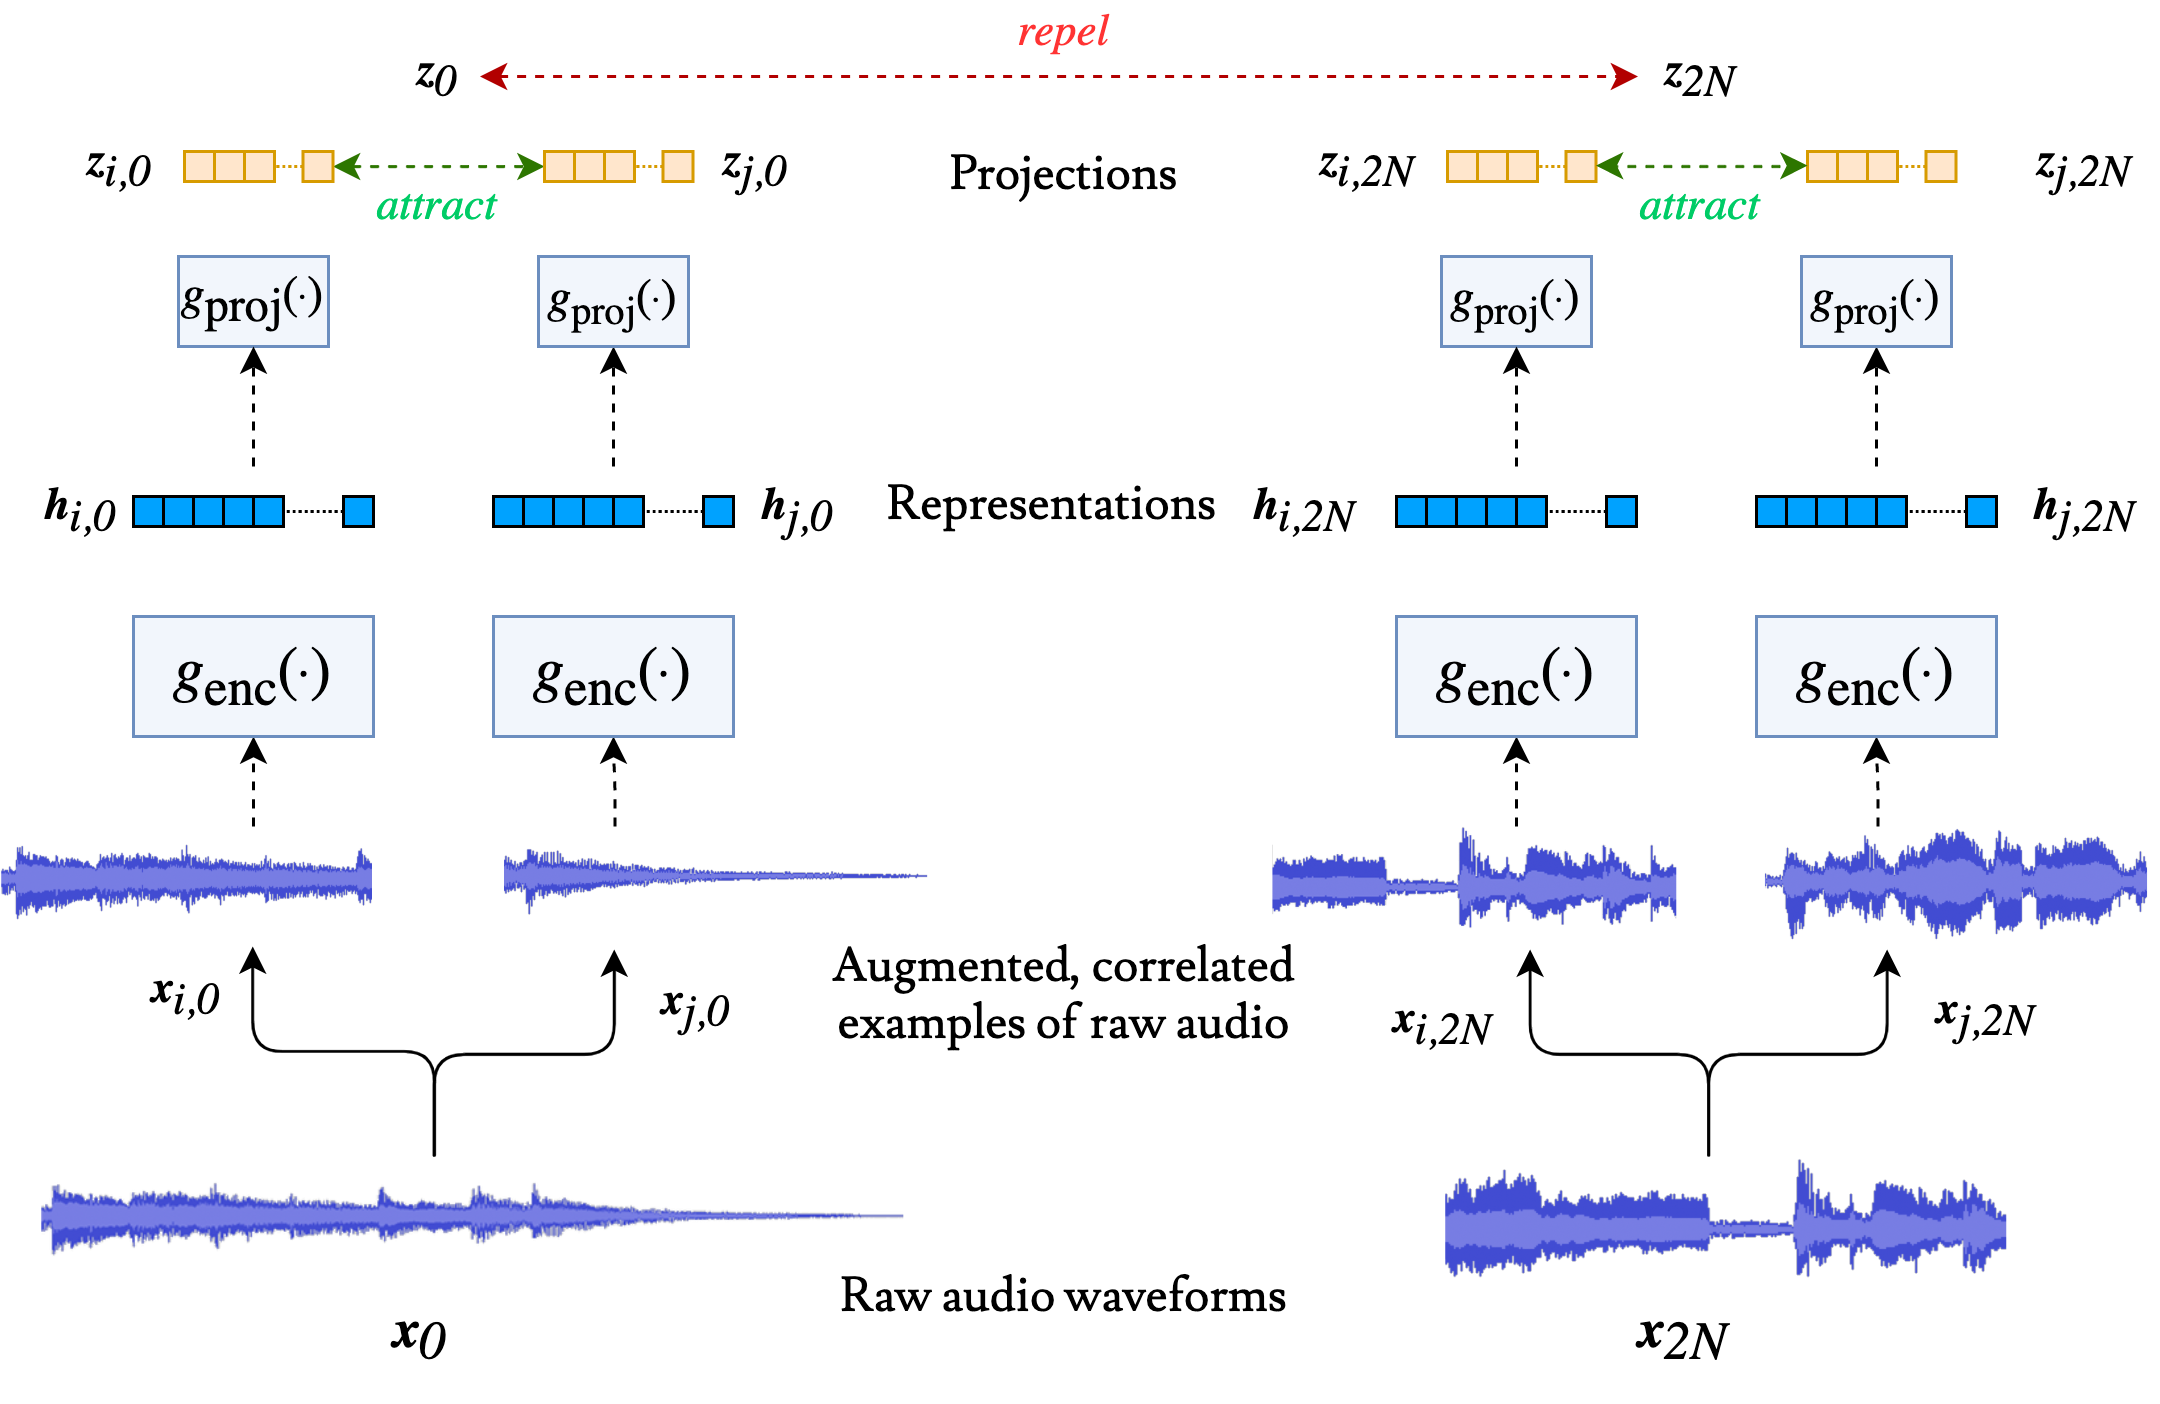
\includegraphics[width=\columnwidth]{figs/clmr_model.png}
    \caption{The proposed contrastive learning framework for audio, in which the contrastive learning objective is directly formulated in the latent space of correlated, augmented examples of the same raw audio waveforms.}
    \label{fig:clmr_model}
\end{figure}


\section{Data Augmentations}
We designed a chain of common augmentations for audio to make it harder for the model to identify the correct pair of examples. The following augmentations were applied on ${x_i}$ and ${x_j}$ independently:
\begin{enumerate}
    \item A random segment of size $N$ is selected from a full piece of audio, without trimming silence (e.g., the intro or outro of a song). The independently chosen segments for $x_i$ and $x_j$ could overlap or be very disjoint, allowing the model to infer both local and global structures.
    \item The polarity is inverted with probability $p_{\mathrm{invert}}$.
    \item Noise is added with probability $p_{\mathrm{noise}}$.
    \item The gain is reduced between $[-6, 0]$ decibels with probability $p_{\mathrm{gain}}$.
    \item A filter is applied with probability $p_{\mathrm{filter}}$. A coin flip determines whether it is a low-pass ($3500$~Hz) or high-pass ($800$~Hz) filter.
\end{enumerate}
The space of augmentations is not limited to these operations and could easily be extended to, e.g., randomly applying pitch shifts, reverberation, delay, chorus and other modulations. When designing a chain of augmentations, however, one must be cautious not to let the model become invariant to potentially important features. \
% \diffword{rephrase example}
For example, when randomly shifting the pitch of the audio, creating two augmented examples of the same segment, 
% with in mind the model's objective is to identify the pair from all the negative examples, 
the model could become invariant to frequency differences.
% which may negatively impact model performance. 
% \diffword{Layer2 is data augment in \ref{clmr}}.


\section{Mini-Batch Composition} % Negative examples
We sample one song from the mini-batch, augment it into two examples, and treat them as the positive pair. We treated the remaining $2(N-1)$ examples in the mini-batch as negative examples, and did not sample the negative examples explicitly. A larger batch size makes the model's objective harder -- there are simply more negative samples -- but it can substantially improve model performance\cite{chen_simple_2020}. The batch size can be increased more easily when audio is re-sampled at lower sampling rates: the number of examples the model is exposed to at once can be higher when the number of audio samples is lower.

Batch normalisation\cite{batch_normalisation} is used in the encoder to stabilise training. When training in a distributed, parallel manner, the batch normalisation statistics (mean/variance) are usually aggregated locally per device. Positive examples are sampled on the same device, leading to potential leakage of batch statistics which improves training loss, but counteracts learning of useful representations. We used global batch normalisation, which aggregates the batch statistics over all devices during parallel training, and leave the effect of different stabilisation strategies, e.g., layer normalisation \cite{henaff2019data}, for future work.


\section{Encoder}
Raw audio waveforms are very high-dimensional: a segment of 3~s already has 66\,150 samples when sampled at 22\,050~Hz, and they convey a lot of information at different time-scales. Architectures with many convolutional layers with small filter sizes have been shown to capture these complexities very well (e.g., SampleCNN \cite{lee2018samplecnn}), generating a feature vector for every sample of audio. Similarly to previous work on music classification of raw waveforms, we use an audio input of $\approx$~2.5 seconds\cite{dieleman2014end,lee2018samplecnn,pons_end--end_2017} and adjust the encoder accordingly when training on audio sampled at different sampling rates (22\,050, 12\,000 and 8\,000~Hz). For a segment length of 59\,049 samples, the encoder $g_{\mathrm{enc}}$ consists of 11 blocks, each with a convolutional layer with a filter size of 3, batch normalisation, ReLU activation and max pooling with pool size 3. The fully connected and dropout layers are removed, yielding a 512-dimensional feature vector for every sample. This feature vector is subsequently mapped to a different latent space by the projector network $g_{\mathrm{proj}}$ where the contrastive loss function is defined.

\subsection{Projector}
The feature vectors from the encoder can be directly used in the learning objective, but SimCLR\cite{chen_simple_2020} shows that formulating the objective on encodings mapped to a different latent space by a parameterised function helps the effectiveness of the representations. We evaluate the performance improvement when using a linear layer $z_i = Wh_i$, non-linear layer $z_i = W^{(2)}\operatorname{ReLU}(W^{(1)}h_i)$ and an identity function $z_i = \mathbbm{1}h_i$ as the projector.
% \diffword{Layer2 is data augment in \ref{clmr}}.


\section{Contrastive Loss Function}
In keeping with recent findings on several objective functions\cite{chen_simple_2020}, the contrastive loss function used in this model is again based on noise-contrastive estimation: normalised temperature-scaled cross-entropy loss, commonly denoted as \emph{NT-Xent loss}:
\begin{equation}
    \label{ntxent_loss}
    \ell_{i, j}=-\log \frac{\exp \left(\operatorname{sim}\left(z_{i}, z_{j}\right) / \tau\right)}{\sum_{k=1}^{2 N} \mathbbm{1}_{[k \neq i]} \exp \left(\operatorname{sim}\left(z_{i}, z_{k}\right) / \tau\right)}
\end{equation}
%, demonstrated for a single pair in equation \ref{ntxent_loss}. 
Instead of using a scoring function that preserves the mutual information between vectors, the pairwise similarity is measured using cosine similarity ($\operatorname{sim}$).
% : $f(\cdot) = \operatorname{sim}(\boldsymbol{u}, \boldsymbol{v})=\boldsymbol{u}^{\top} \boldsymbol{v} /\|\boldsymbol{u}\|\|\boldsymbol{v}\|$.
It introduces a new temperature parameter $\tau$ to help the model learn from hard negatives. The indicator function $\mathbbm{1}_{[k \neq i]}$ evaluates to $1$ iff $k\neq i$.
% ref to figure
This loss is computed for all pairs, both $(z_i, z_j)$ and $(z_j, z_i)$, resulting in the following total loss function:
% shown in equation \ref{total_xent_loss}.

\begin{equation}
    \label{total_xent_loss}
    \mathcal{L} = \frac{1}{2N}\sum_{i=1}^{N}\sum_{j=1}^{N} \mathbbm{1}_{[i\neq j]}\ell_{i, j}
\end{equation}

There is a trade-off between the number of contrastive examples the model is exposed to at once, and model complexity: increasing both quickly results in hardware constraints for training (GPU memory). We found working with a batch size of 48 and a $3^9$-SampleCNN encoder to work well and easier to compare with against related work using supervised methods \cite{lee2018samplecnn, dieleman2014end,pons_end--end_2017}. We leave model scaling for future work. We used the Adam optimizer \cite{adam_optimizer} with a learning rate of $3\times10^{-4}$ and train until convergence.

\section{Evaluation}
\label{evaluation}
The evaluation of representations learned by self-supervised models is commonly done with linear evaluation \cite{oord_representation_2019,hjelm_learning_2019,chen_simple_2020}, which measures how linearly separable the relevant classes are under the learned representations. We obtain representations for all data points $X$ after pre-training has converged, and train a multi-class, linear logistic regression model. For CPC, the representations are extracted from the autoregressor, yielding context vector $c$ of $256$ dimensions, which is global-average pooled to obtain a single vector of $512$ dimensions. For CLMR, the representations $h$ from the encoder are used instead of the representations $z$ from the projector. 


\section{Transfer Learning}
To test the generalisability of the learned representations, we also pre-trained CLMR and CPC on different datasets than those we use for evaluation. There are no overlapping songs between datasets. All datapoints $X$ from the evaluation dataset were processed through a frozen, converged network to obtain representations $h$, on which we perform the same linear evaluation procedure outlined in the previous paragraph. 


\chapter{Experimental Results}
\begin{table}[t]
    \centering
    \ra{1.3}
    \resizebox{\columnwidth}{!}{
    \begin{tabular}{@{}llcc@{}}\toprule
        Model & Train Dataset & ROC-AUC & PR-AUC \\ \midrule
        \multicolumn{4}{c}{MTAT-Trained Experiments}\\\addlinespace
        Pons et al.$^\dagger$ & MTAT & \textit{89.05} & \textit{34.92} \\
        SampleCNN$^\dagger$ & MTAT & 88.56 & 34.38 \\
        CLMR (ours) & MTAT & \textbf{87.03} (87.56) & \textbf{31.76} (32.73) \\
        CPC (ours) & MTAT & 86.60 (\underline{87.99}) & 30.98 (\underline{33.04}) \\
        1D CNN$^\dagger$ & MTAT & 85.58 & 29.59 \\\midrule
        \multicolumn{4}{c}{Transfer Learning Experiments}  \\\addlinespace
        CPC & FMA & \textbf{86.34} (\underline{87.79}) & \textbf{30.71} (\underline{32.47}) \\
        CLMR & FMA & 86.22 (86.63) & 30.58 (31.22) \\
        CPC & Billboard & 85.78 (86.25) & 29.68 (30.15) \\
        CPC & GTZAN & 83.44 (86.06) & 26.88 (29.72) \\
        CLMR & Billboard & 82.73 (84.22) & 26.86 (27.82) \\
        CLMR & GTZAN & 81.88 (85.43) & 26.18 (29.49) \\
        \bottomrule
        \end{tabular}
    }
    \caption{Tag prediction performance on the MagnaTagATune (MTAT) dataset, compared with fully supervised models$^\dagger$ trained on raw audio waveforms. The ROC-AUC and PR-AUC scores are tag-wise scores obtained by end-to-end training for the supervisd models. For the self-supervised models, the scores are obtained by training a \emph{linear}, logistic regression classifier on the MTAT dataset using the representations from self-supervised pre-training. Scores in parenthesis show performance when adding one hidden layer to the logistic regression classifier, making it a simple multi-layer perceptron. Transfer learning experiments show the performance of the self-supervised models when pre-trained on datasets different from the evaluation dataset, again using a linear classifier to evaluate.}
    \label{tab:magnatagatune_results}
\end{table}



\section{Datasets}
We evaluated the quality of our models' representations with music classification experiments. We used the MagnaTagATune\cite{law2009evaluation} dataset for training and evaluation, and additionally used the fault-filtered GTZAN\cite{tzanetakis2002musical,sturm2013gtzan}, McGill Billboard\cite{burgoyne_billboard} and Free Music Archive\cite{fma_dataset} datasets to perform pre-training for transfer learning. 

Predicting the top~50 tags in the Magna\-Tag\-A\-Tune dataset is a popular benchmark for music classification. It is a multi-label classification task: each track can have multiple tags from a set of 188 in total, of which we use the 50 most frequently occuring to compare our performance against supervised benchmarks. 
We used the original, MIREX 2009 version of the dataset, consisting of 25\,863 songs, and the same dataset split, so that we can compare our results with previous work\cite{pons_end--end_2017, lee2018samplecnn, dieleman_feature_learning} easily. It should be noted that this original version contains tag labels that are synonymous, e.g., `female', `woman', `no vocal', `no voice' and also contains tracks with no labels.
Like other studies, we use average tag-wise ROC-AUC and PR-AUC scores as evaluation metrics, global measures indicating how well the classifier ranks segments given a tag. PR-AUC is calculated in addition to ROC-AUC because ROC-AUC scores can be over-optimistic for imbalanced datasets like MagnaTagATune\cite{pons_end--end_2017}. 

From the McGill Billboard dataset, we use 461 audio files of contemporary pop songs for training. While this dataset is most often used for evaluating chord recognition algorithms, we use it solely for self-supervised pre-training.
Similarly, we use the Free Music Archive dataset, consisting of 22\,413 unique songs for the `medium' version, also for self-supervised pre-training only. The fault-filtered GTZAN dataset contains 930 songs of 30 seconds, each having a single label denoting the segment's genre.

\section{Quantitative and Qualitative Evaluation}
The evaluation metrics for the best-performing models are shown in Table \ref{tab:magnatagatune_results}. Both CPC and CLMR show competitive performance with fully supervised models in the music classification task, despite being pre-trained without ground truth and using a simple, linear classifier for evaluation. A non-linear projector network positively impacts the performance of the model. Adding only one extra hidden layer to the classifier increases the results by $4\%$, making the gap between supervised end-to-end baselines even smaller.
% It is clear from these results that useful representations can be learned from high-dimensional signals of raw audio even without access to ground truth labels. 

For a qualitative view of the representations, we show how cleanly they are  separable using a $t$-SNE manifold in Figure \ref{fig:tsne_manifold}. Figure \ref{fig:tag_scores} shows in more detail that the difference in performance between self-supervised and supervised models is marginal: there is no single tag performance difference larger than 4\% ROC-AUC, and for practical purposes, CLMR and CPC retrieve tags practically identically to supervised models.

\begin{figure}[t]
    \centering
    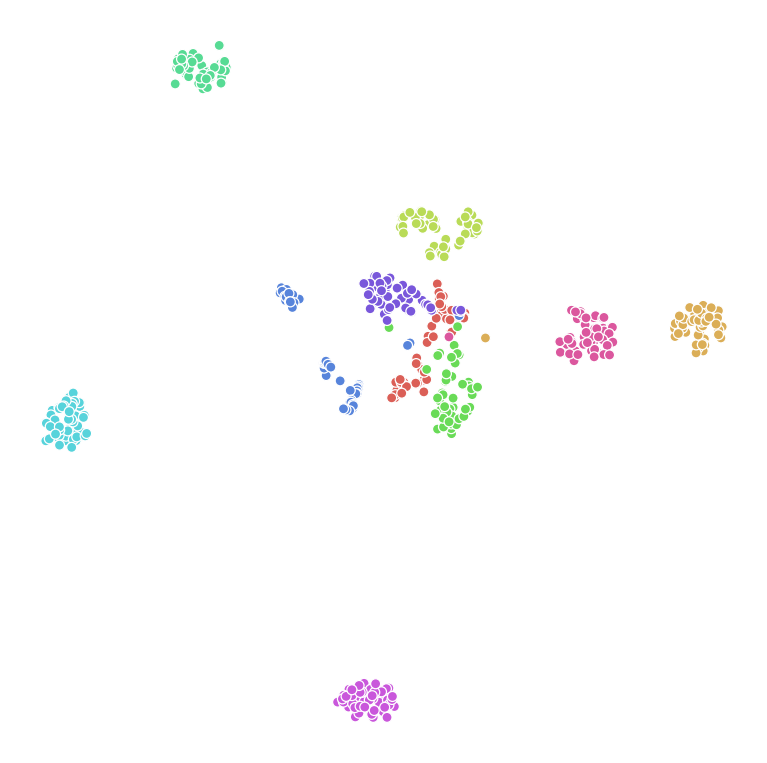
\includegraphics[width=0.75\columnwidth]{figs/tsne-clmr.png}
    \caption{$t$-SNE manifold visualisation from audio representations learned by a converged CLMR model of a subset of 10 tracks with each 60 segments, }
    \label{fig:tsne_manifold}
\end{figure}

\begin{figure*}[t]
    \centering
    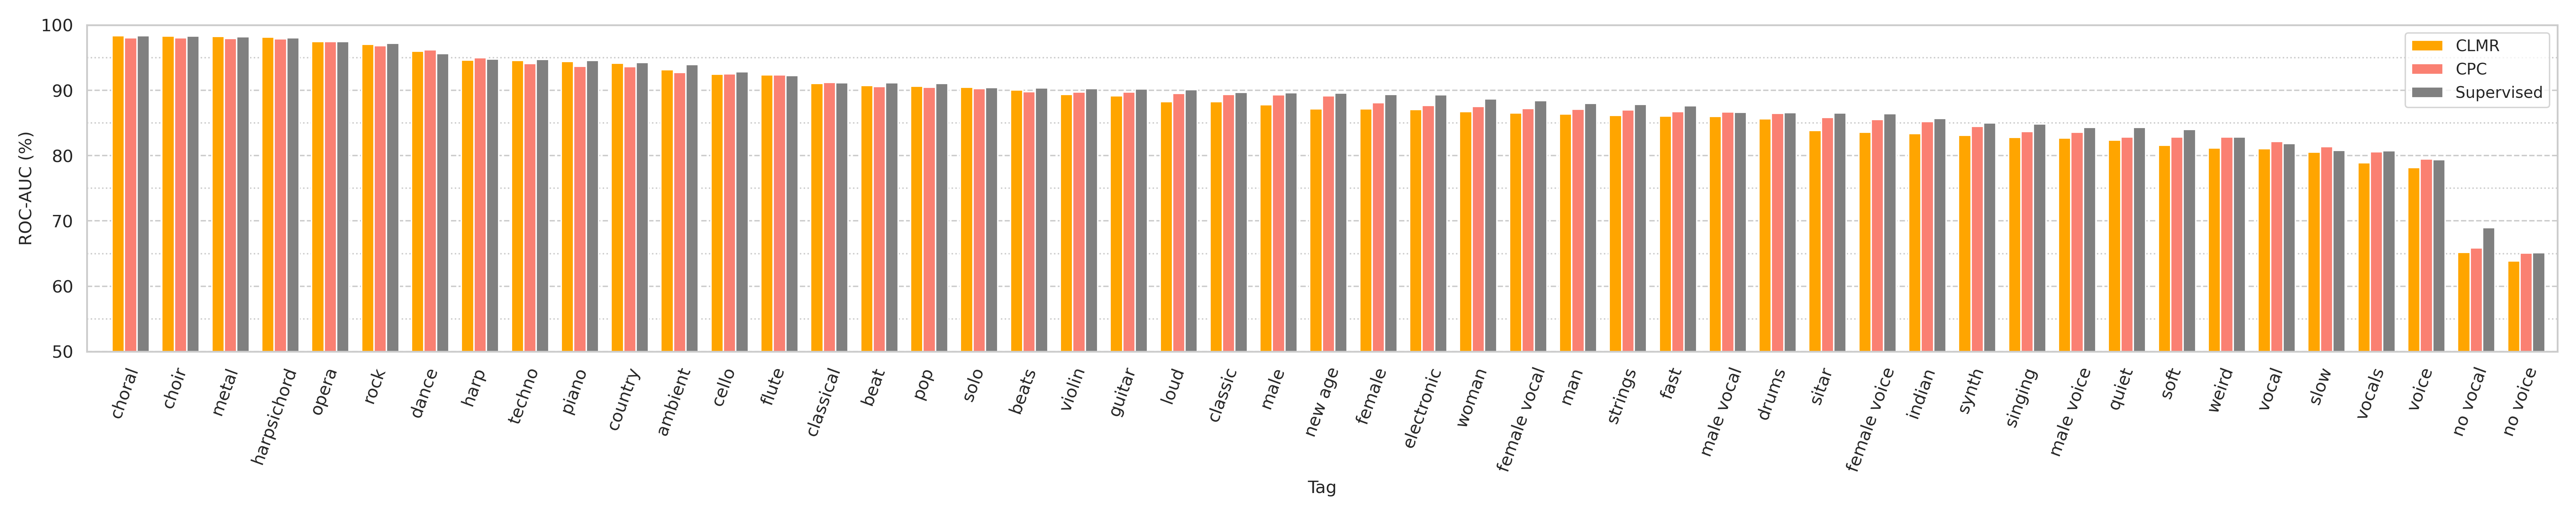
\includegraphics[width=\textwidth]{figs/tag_retrieval.png}
    \caption{Tag-wise ROC-AUC scores for the top-50 tags in the MagnaTagATune dataset, reported for linear, logistic regression classifiers trained on representations of self-supervised models CLMR and CPC, and compared to a fully supervised, end-to-end SampleCNN model.}
    \label{fig:tag_scores}
\end{figure*}


\begin{figure*}[t]
    \centering
    \subcaptionbox{CLMR$^{(1)}_{\mathrm{MTAT}}$\label{fig:1a}}{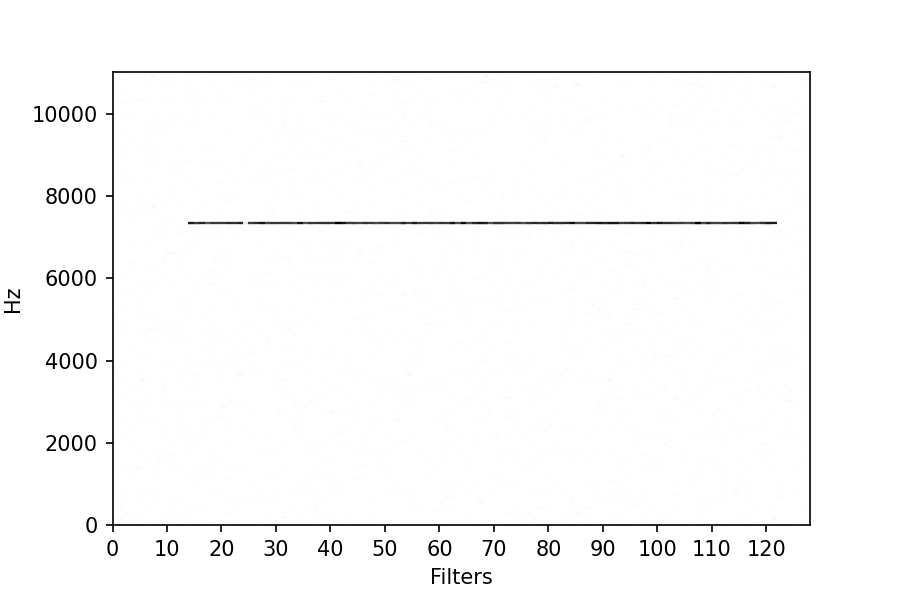
\includegraphics[width=.16\textwidth]{figs/magnatagatune/clmr_spectrum/epoch1490_layer0.png}}\hfill
    \subcaptionbox{CLMR$^{(4)}_{\mathrm{MTAT}}$\label{fig:1a}}{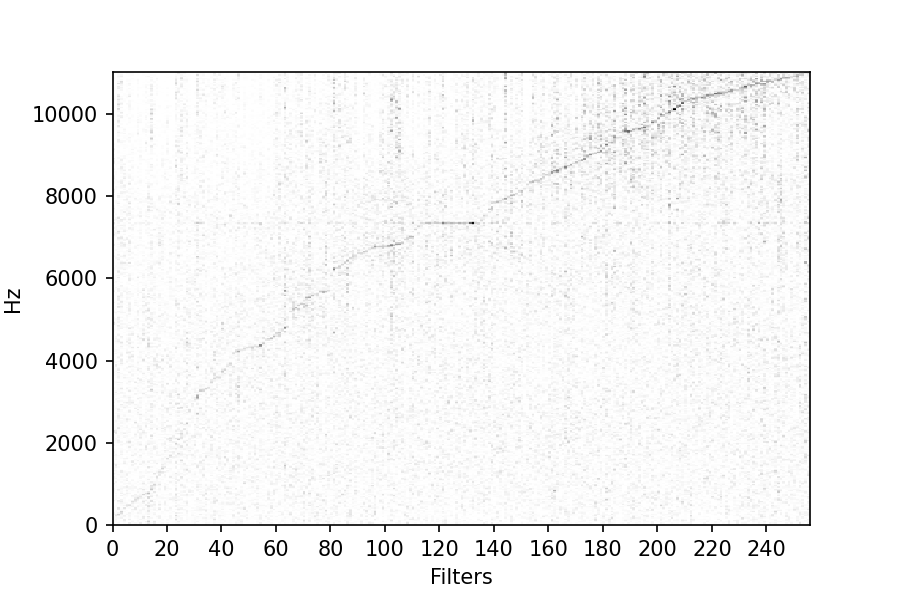
\includegraphics[width=.16\textwidth]{figs/magnatagatune/clmr_spectrum/epoch1490_layer3.png}}\hfill
    \subcaptionbox{CLMR$^{(6)}_{\mathrm{MTAT}}$\label{fig:1a}}{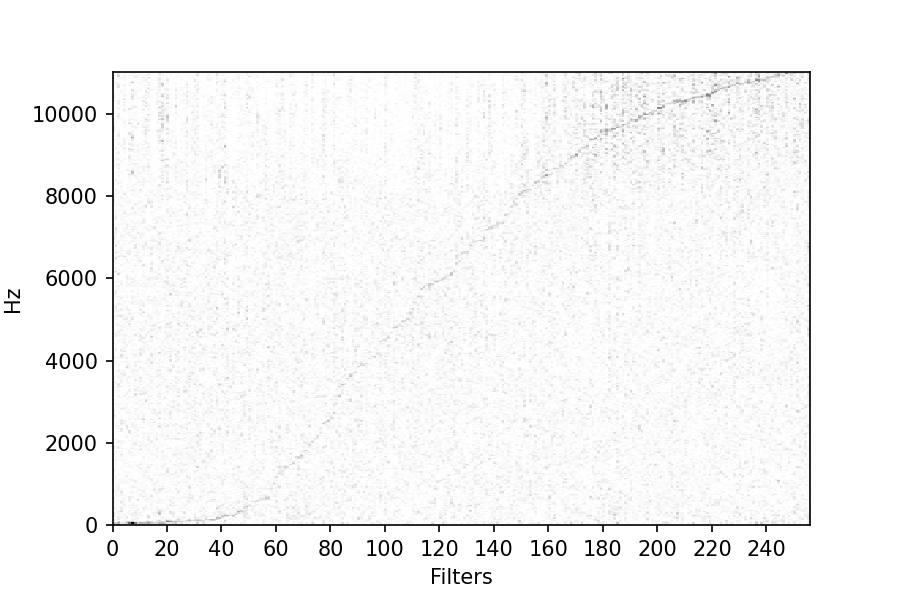
\includegraphics[width=.16\textwidth]{figs/magnatagatune/clmr_spectrum/epoch1490_layer5.png}}\hfill
    \subcaptionbox{CPC$^{(1)}_{\mathrm{MTAT}}$\label{fig:1a}}{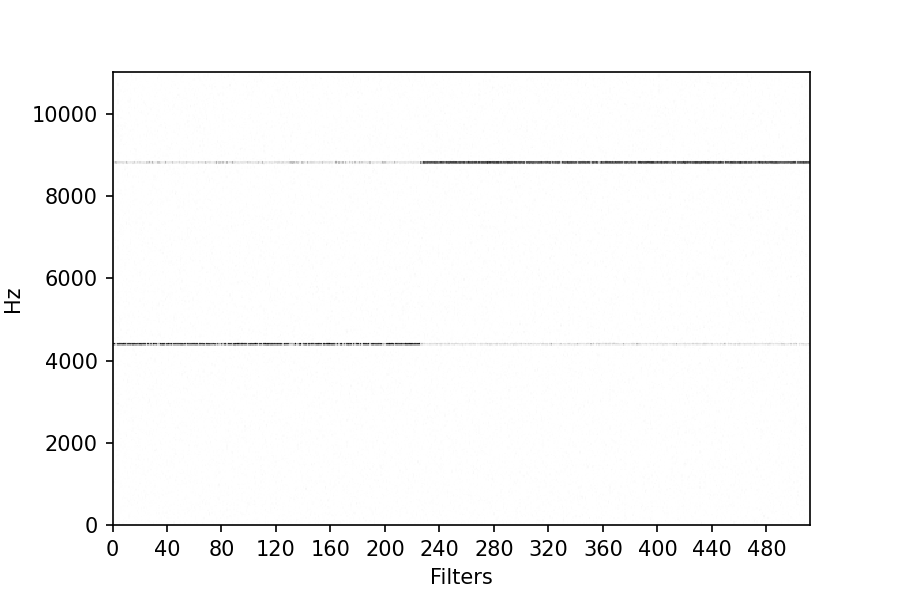
\includegraphics[width=.16\textwidth]{figs/magnatagatune/cpc_spectrum/epoch670_layer0.png}}\hfill
    \subcaptionbox{CPC$^{(4)}_{\mathrm{MTAT}}$\label{fig:1a}}{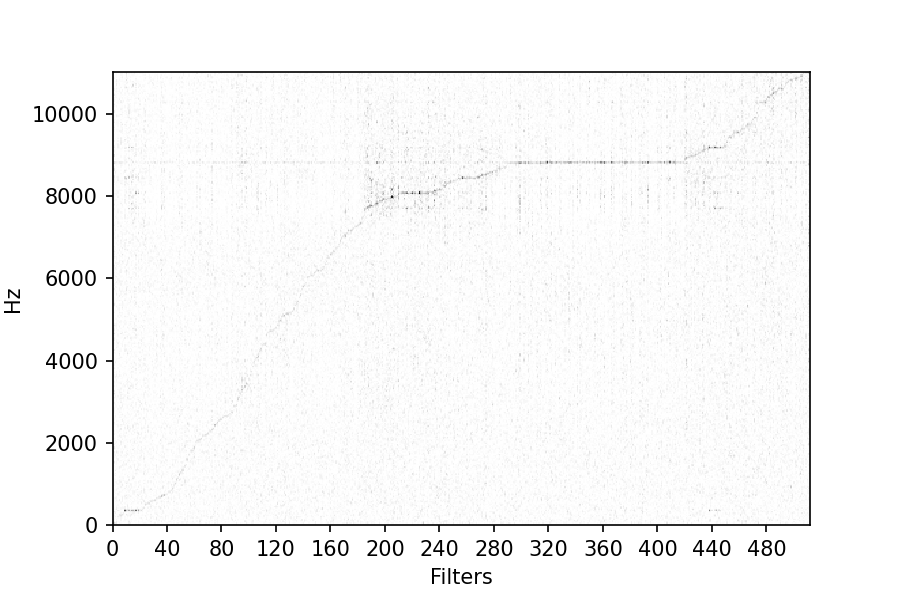
\includegraphics[width=.16\textwidth]{figs/magnatagatune/cpc_spectrum/epoch670_layer3.png}}\hfill
    \subcaptionbox{CPC$^{(6)}_{\mathrm{MTAT}}$\label{fig:1a}}{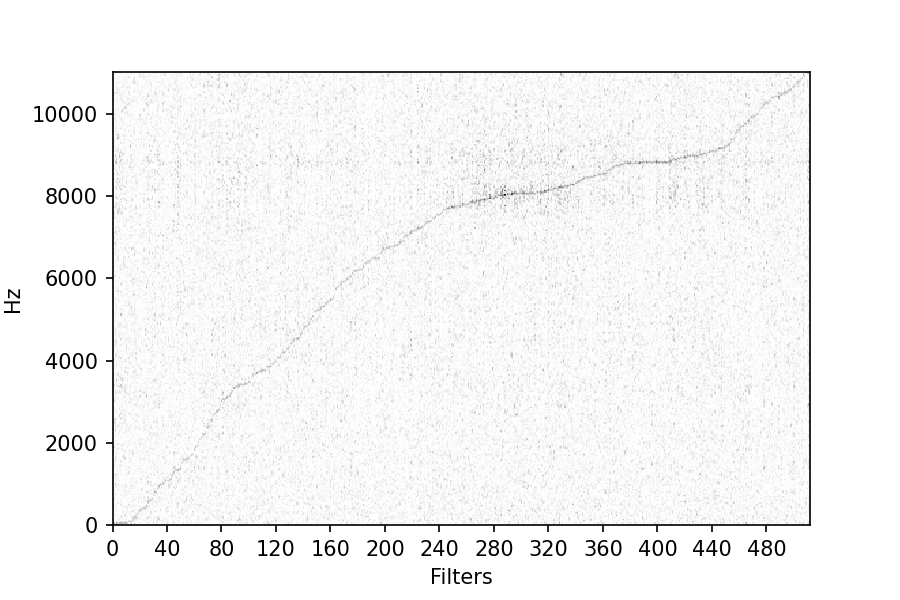
\includegraphics[width=.16\textwidth]{figs/magnatagatune/cpc_spectrum/epoch670_layer5.png}}

    \subcaptionbox{CLMR$^{(1)}_{\mathrm{Billboard}}$\label{fig:1a}}{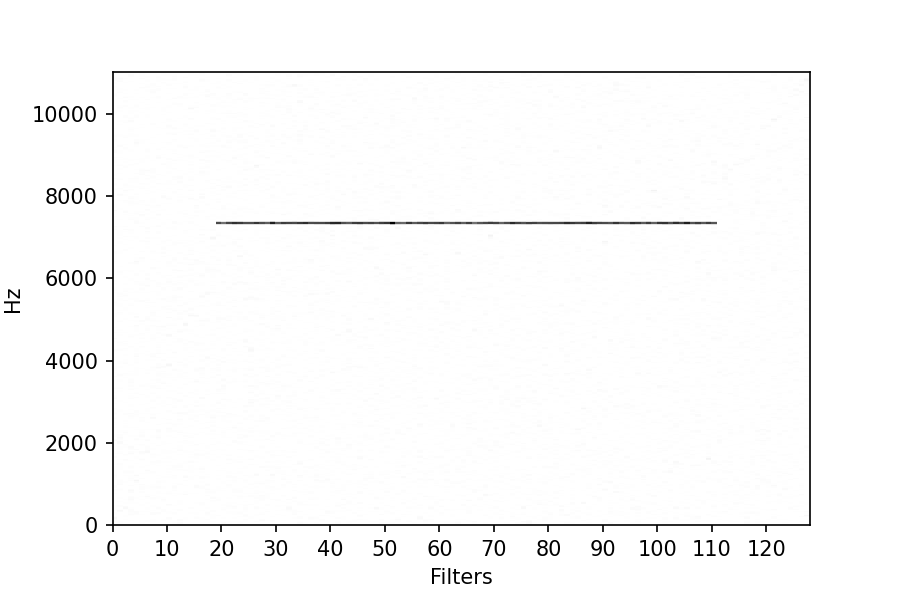
\includegraphics[width=.16\textwidth]{figs/billboard/clmr_spectrum/epoch1490_layer0.png}}\hfill
    \subcaptionbox{CLMR$^{(4)}_{\mathrm{Billboard}}$\label{fig:1a}}{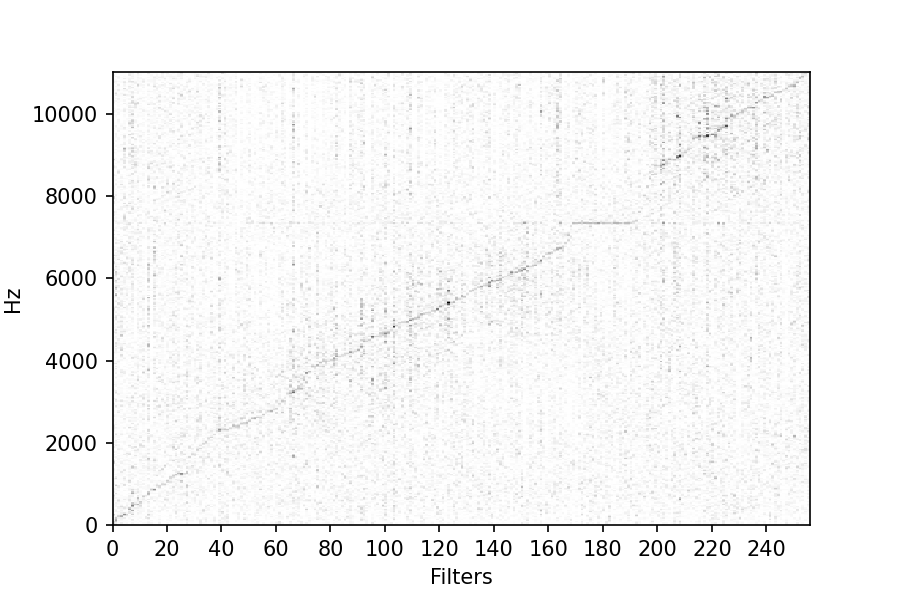
\includegraphics[width=.16\textwidth]{figs/billboard/clmr_spectrum/epoch1490_layer3.png}}\hfill
    \subcaptionbox{CLMR$^{(6)}_{\mathrm{Billboard}}$\label{fig:1a}}{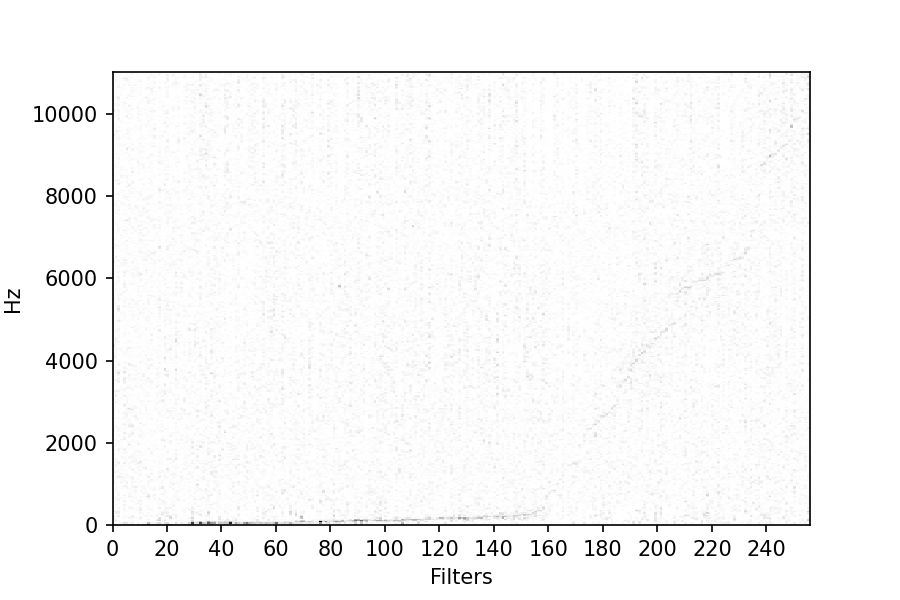
\includegraphics[width=.16\textwidth]{figs/billboard/clmr_spectrum/epoch1490_layer5.png}}\hfill
    \subcaptionbox{CPC$^{(1)}_{\mathrm{Billboard}}$\label{fig:1a}}{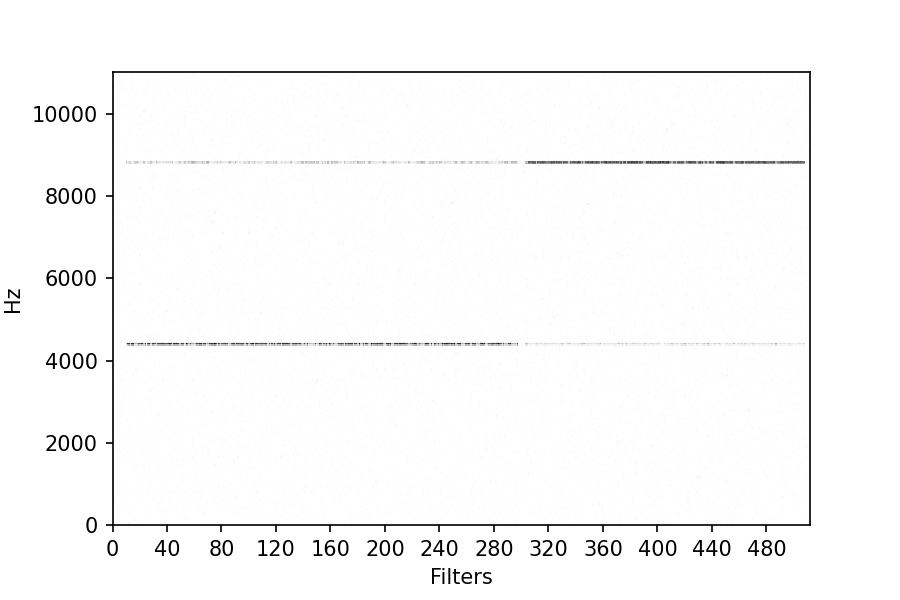
\includegraphics[width=.16\textwidth]{figs/billboard/cpc_spectrum/epoch1490_layer0.png}}\hfill
    \subcaptionbox{CPC$^{(4)}_{\mathrm{Billboard}}$\label{fig:1a}}{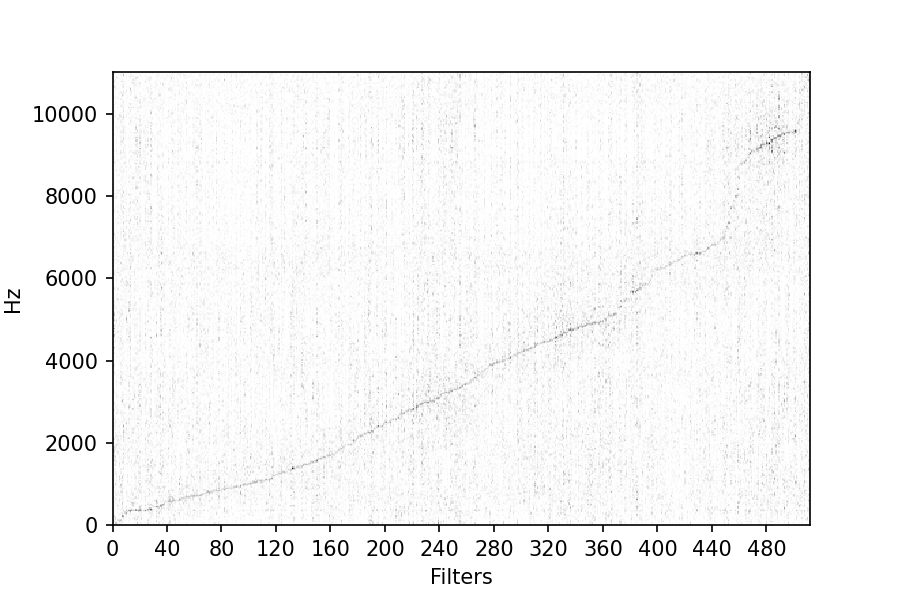
\includegraphics[width=.16\textwidth]{figs/billboard/cpc_spectrum/epoch1490_layer3.png}}\hfill
    \subcaptionbox{CPC$^{(6)}_{\mathrm{Billboard}}$\label{fig:1a}}{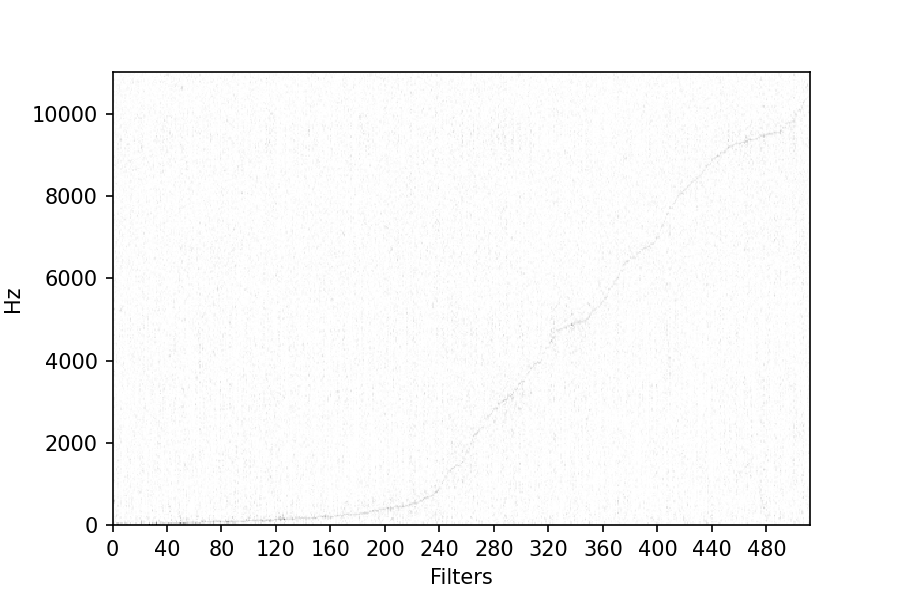
\includegraphics[width=.16\textwidth]{figs/billboard/cpc_spectrum/epoch1490_layer5.png}}

    \caption{Normalised magnitude spectrum of the filters of the self-supervised models in the sample-level convolution layers, sorted by the frequency of the peak magnitude. Gradient ascent is performed on a randomly initialised waveform of 729 samples (close to typical frame size) and its magnitude spectrum is calculated subsequently. Each vertical line in the graph represents the frequency spectrum of a different filter. The first three images are taken from a pre-trained, converged CLMR model, the last three from a CPC model, on the MTAT or Billboard datasets}
    \label{fig:filter_visualisation}
\end{figure*}


\section{Data Augmentations and Mini-Batch Size}
Our results show that all data augmentations, with the exception of adding random noise, contribute to a higher accuracy score. Using $p_{\mathrm{filter}}=0.4$ increases PR-AUC by $5.5\%$, and the performance difference is $8\%$ when all augmentations are done instead of only random trimming. When re-sampling the audio to 8\,000~Hz and 12\,000~Hz respectively, there is a marginal penalty to the final accuracy scores for the self-supervised models, which is in line with previous work\cite{lee2018samplecnn}. Increasing the batch size to 192 and 128 respectively also increases final evaluation scores. We refer the reader to the supplementary material for a complete overview of the results obtained with different augmentation and model parameters.

\section{Transfer Learning}
The results of the transfer learning experiments are shown in Table \ref{tab:magnatagatune_results}. Both CPC and CLMR show the ability to learn effective representations from datasets different from the evaluation dataset without ground truth, and even exceed accuracy scores of previous, supervised end-to-end systems on raw audio\cite{dieleman2014end}. Moreover, both models demonstrate the ability to learn useful representations on small datasets like GTZAN. The CLMR model performs better when pre-trained on larger datasets, which is expected as it heavily relies on the number of unique, independent examples to create correlated augmentations. When pre-training on smaller datasets, the autoregressive modelling in CPC can find more useful representations for downstream tasks.
%contribute to more useful representations for downstream tasks.



\section{Visualising filters}
Figure \ref{fig:filter_visualisation} shows the magnitude spectrum of the learned filters of the sample-level convolutional layers (layers 1, 4 and 6) for CLMR and CPC, pre-trained on the MTAT and Billboard dataset. In CLMR, the first layer is sensitive to a single, very small band of frequencies around 7500~Hz, while in higher layers, the filters spread themselves first linearly and then non-linearly across the full range. CPC shows a similar pattern in the lowest layer, but shows a strong activation of two frequencies that span an octave. Interestingly, CLMR shows a similar filter structure for the Billboard data set as fully supervised models that were trained on the MTAT dataset \cite{dieleman2014end,lee2018samplecnn}. The Billboard dataset is significantly less diverse in genre, suggesting the self-supervised model focuses more on such frequency-band related differences than it does for the more diverse Magna\-Tag\-A\-Tune.




\chapter{Conclusion}
In this paper, we presented CLMR, a self-supervised contrastive learning framework that learns useful and compact representations of raw waveforms of musical audio. The framework requires no preprocessing of the input and is trained without ground truth, which enables simple and straightforward pre-training on datasets of unprecedented scale. We tested the representations in the music classification task on the MagnaTagATune dataset, achieving competitive performance with state-of-the-art supervised models, exceeding previous supervised benchmarks, and demonstrated the transferability of representations learned from pre-training on different datasets. The simplicity of training the model without a direct supervised signal and without preprocessing inputs, together with encouraging results obtained with a single linear layer optimised for a challenging downstream task, are exciting developments towards unsupervised learning on raw musical signals.



\bibliographystyle{unsrt}
\bibliography{bibliography}


\chapter*{Supplemental Material}


\begin{table*}[h]
    \centering
    \resizebox{\textwidth}{!}{
        \begin{tabular}{c|c|c|c|c|c|c|c|c|c|c|c|c}
        batch size & audio length & sample rate & projector dim. & temperature & $p_{\mathrm{invert}}$ & $p_{\mathrm{noise}}$ & $p_{\mathrm{gain}}$ & $p_{\mathrm{filter}}$ & ROC-AUC$^{(\mathrm{MLP})}$ & PR-AUC$^{(\mathrm{MLP})}$ \\ \hline
        48 & 59049 & 22050 & 128 & 0.1 & 0.8 & 0.5 & 0.1 & 0.4 & \textbf{87.56} & 32.25 \\
        48 & 59049 & 22050 & 128 & 0.5 & 0.8 & 0.5 & 0.1 & 0.4 & 87.55 & 32.66 \\
        192	& 20736 & 8000 & 128 & 0.5 & 0.8 & 0.5 & 0.1 & 0.4 & 87.52 & 32.43 \\
        48	& 20736 & 8000 & 128 & 0.5 & 0.8 & 0.5 & 0.1 & 0.4 & 87.49 & 32.38 \\
        48 & 59049 & 22050 & 256 & 0.5 & 0.8 & 0.5 & 0.1 & 0.4 & 87.43 & 32.58 \\
        48 & 59049 & 22050 & 64	& 0.5 & 0.8 & 0.5 & 0.1 & 0.4 & 87.43 & 32.49 \\
        128 & 31104 & 12000	& 128 & 0.5 & 0.8 & 0.5 & 0.1	& 0.4 & 87.41 & \textbf{32.73} \\
        48 & 31104 & 12000 & 128 & 0.5 & 0.8 & 0.5 & 0.1 & 0.4 & 87.37 & 32.69 \\
        48 & 59049 & 22050 & 128 & 0.25 & 0.8 & 0.5 & 0.1 & 0.4 & 87.36 & 32.42 \\
        48 & 59049 & 22050 & 128 & 0.5 & 0.8 & 0.5 & 0.1 & 0.4 & 87.00 & 31.93 \\
        48 & 59049 & 22050 & 128 & 0.5 & 0.8 & 0.5 & 0.1 & 0 & 85.99 & 30.26 \\
        48 & 59049 & 22050 & 128 & 0.5 & 0.8 & 0 & 0 & 0 & 85.79 & 30.55 \\
        48 & 59049 & 22050 & 128 & 0.5 & 0.8 & 0.5 & 0 & 0 & 85.67 & 30.03 \\
        48	& 59049	& 22050	& 128 & 0.5	& 0 & 0 & 0 & 0	& 85.54 & 29.84 \\
        \end{tabular}
    }
    \caption{Ablation study of CLMR under different parameters, sampling rate and data augmentations. The ROC-AUC and PR-AUC scores are obtained with a logistic regression classifier with one hidden layer, and is trained only on the representations from a pre-trained, frozen CLMR network.}
    \label{tab:1}
  \end{table*}

\end{document}